\documentclass[a4paper,11pt,exos]{nsi} % COMPILE WITH DRAFT
\usepackage{pifont}
\usepackage{fontawesome5}
\usepackage{hyperref}



\begin{document}
\classe{\terminale Comp}
\titre{Exo - Fonction logarithme népérien}
\maketitle

\tabularstyled[UGLiBlue]
\begin{tabular}{p{16.5cm}}
    \rowcolor{UGLiBlue}
    \ths Capacités attendues : \\

    \ding{111} Utiliser l’équation fonctionnelle du logarithme pour transformer une écriture, résoudre une équation, une inéquation.  \\
    \ding{111} 	Utiliser la relation $\ln q^n= n\ln q$ pour déterminer un seuil.\\
    \ding{111} Dans le cadre de la résolution de problème, utiliser le calcul des limites, l’allure des courbes représentatives de la fonction logarithme.
\end{tabular}


\vspace*{1cm}
\subsection*{Définition de la fonction logarithme népérien}

\exo{} %Indice p 85
\begin{enumerate}
    \item Pour quelles valeurs de $x$, $\ln(x)$ est-il défini ?
    \item Donner la valeur de $e^{\ln 7}$.
    \item Donner la valeur de $\ln(e^5)$ et de $\ln(e^{-3})$.
    \item On note $\mathcal{C}$ la courbe représentative de la fonction $\ln$ dans un repère orthonormé.\\
    Indiquer si les affirmations suivantes sont vraies ou fausses :
    \begin{enumalph}
        \item $\mathcal{C}$ est au-dessus de l'axe des abscisses.
        \item $\mathcal{C}$ passe par le point de coordonnées $(1,0)$.
    \end{enumalph}
\end{enumerate} 

\exo{} %Indice p 85
Simplifier les expressions suivantes :
\begin{multicols}{3}
    \begin{enumerate}
        \item $\dfrac{\ln\left(e^{-2}\right)}{\ln\left(e^4\right)}$
        \item $\ln\left(e^9\right)\times\ln\left(e^{-2}\right)$
        \item $\ln\left(e\right)+\ln\left(\dfrac{1}{e}\right)$
        %\item $\ln\left(\dfrac{1}{e}\right)+\ln\left(\dfrac{1}{e^2}\right)$
    \end{enumerate}
\end{multicols}

\exo{}
Parmi les courbes suivantes, quelle est la représentation graphique de la fonction $\ln$ ?
\begin{center}
    \def\xmin{-3} \def\ymin{-3}\def\xmax{8}\def\ymax{3}
		\begin{tikzpicture}[scale=.7]
			\clip (\xmin,\ymin) rectangle (\xmax,\ymax);
			\draw[fill = white] (\xmin,\ymin) rectangle (\xmax,\ymax);
			\repereal{\xmin}{\ymin}{\xmax}{\ymax}
			\draw[color=UGLiRed,thick,samples=1000,domain=0.01:\xmax,smooth,variable=\x] plot ({\x},{ln(\x)});
            \draw[color=UGLiBlue,thick,samples=1000,domain=-1.99:\xmax,smooth,variable=\x] plot ({\x},{ln(\x+2)});
            \draw[color=UGLiGreen,thick,samples=1000,domain=1.01:\xmax,smooth,variable=\x] plot ({\x},{ln(-1+\x)});
            \draw[color=UGLiOrange,thick,samples=1000,domain=0.01:\xmax,smooth,variable=\x] plot ({\x},{-(\x-2)^2+1});
		\end{tikzpicture}
\end{center}

\exo{}
Sans les calculer, déterminer le signe de chacun des nombres suivants :
\begin{multicols}{3}
    \begin{enumerate}
        \item $\ln\left(8\right)$
        \item $\ln\left(0,1\right)$
        \item $\ln\left(\dfrac{1}{6}\right)$
        \item $\ln\left(1,9\right)$
        \item $\ln\left(100\right)$
        \item $\ln\left(2\times 10^{-3}\right)$
    \end{enumerate}
\end{multicols}

\exo{}
Dans chaque cas, pour quelles valeurs de $x$, les expressions suivantes sont-elles définies ?
\begin{multicols}{3}
    \begin{enumerate}
        \item $\ln\left(x-5\right)$
        \item $\ln\left(6-3x\right)$
        \item $\ln\left(x\right)+\ln\left(4-x\right)$
    \end{enumerate}
\end{multicols}

\subsection*{Résoudre des équations et des inéquations}
\exo{}
\begin{enumerate}
    \item On sait que $e^x=5$. Que vaut $x$ ?
    \item On sait que $\ln(x)=0$. Que vaut $x$ ?
    \item On sait que $\ln(x)=9$. Que vaut $x$ ?
    \item On sait que $\ln(x)=-3$. Que vaut $x$ ?
\end{enumerate}

\exo{}
Résoudre les équations suivantes dans $\oio{0}{+\infty}$ :
\begin{multicols}{4}
    \begin{enumerate}
        \item $\ln(x)=1$
        \item $\ln(x)=7$
        \item $\ln(x)=-2$
        \item $\ln(x)=-1$
    \end{enumerate}
\end{multicols}

\exo{}
Résoudre les équations suivantes dans $\oio{0}{+\infty}$ :
\begin{multicols}{4}
    \begin{enumerate}
        \item $\e^{x}=10$
        \item $3e^x+5=14$
        \item $\ln(2x)+1=0$
        \item $\ln(x)=\ln(2x+1)$
    \end{enumerate}
\end{multicols}

\exo{}
Dans chaque cas, déterminer l'ensemble des nombres réels $x$ pour lesquels les expressions sont bien définies puis résoudre l'inéquation :
\begin{multicols}{4}
    \begin{enumerate}
        \item $\ln(x)\leqslant 2$
        \item $\ln(3x)\geqslant \ln(6)$
        \item $\ln(1-x)> 0$
        \item $\ln(3-2x)\leqslant 1$
        \item $\ln(x-4)\leqslant \ln(1+2x)$
        \item $\ln(x^2-9)>\ln(2)$
        \item $3e^x-1<8$
        \item $e^{2x}-3e^x\geqslant 0$
    \end{enumerate}
    
\end{multicols}



\exo{ \faStar}
On veut résoudre l'équation $\quad e^{2x}-2e^x=8\ (E)$.
\begin{enumerate}
    \item On pose $y=e^x$. Montrer que l'équation précédente est équivalente à $y^2-2y-8=0\ (E')$.
    \item Résoudre l'équation $(E')$.
    \item En déduire les solutions de l'équation initiale $(E)$.
\end{enumerate}

\subsection*{Propriétés algébriques du logarithme népérien}
\exo{}
Exprimer les nombres suivants en fonction de $\ln 2$.
\begin{multicols}{4}
    \begin{enumerate}
        \item $\ln 4$
        \item $\ln 8$
        %\item $\ln 16$
        \item $\ln \dfrac{1}{2}$
        \item $\ln \dfrac{1}{8}$
        \item $\ln (8e)$
        \item $\ln \left(4e^2\right)$
        \item $\ln \sqrt{2}$
        \item $\ln \sqrt{32}$
    \end{enumerate}
\end{multicols}

\exo{}
Écrire les nombres suivants en utilisant une seule fois le symbole $\ln$.
\begin{multicols}{2}
    \begin{enumerate}
        \item $A= 5\ln 2+\ln 8-\ln 4$
        \item $B=2\ln 3+\ln 81-\ln 9$
        \item $C=\ln 3-\ln 2+\ln 5$
        \item $D=\ln 14-\ln 19$
    \end{enumerate}
\end{multicols}

\exo{}
\begin{enumerate}
    \item Écrire le réel $\ln 7 +\ln 2$ en utilisant une seule fois le symbole $\ln$.
    \item En déduire les solution de l'équation $\ln x=\ln 7 +\ln 2$ dans $\oio{0}{+\infty}$.
\end{enumerate}

\exo{}
On considère l'équation $(E) : \ln(x)+ \ln(2x)=\ln(18)$ pour $x$ appartenant à $\oio{0}{+\infty}$.
\begin{enumerate}
    \item Montrer que l'équation $(E)$ est équivalente à $x^2=9$ pour $x>0$.
    \item En déduire l'ensemble des solutions de l'équation $(E)$.
\end{enumerate}

\exo{ \faStar}
On veut résoudre l'équation $\quad \left(\ln x\right)^2+4\ln \dfrac{1}{x}-5=0\ (E)$.
\begin{enumerate}
    \item On pose $y=\ln x$. Montrer que l'équation précédente est équivalente à $y^2-4y-5=0\ (E')$.
    \item Résoudre l'équation $(E')$.
    \item En déduire les solutions de l'équation initiale $(E)$.
\end{enumerate}

\exo{}
Dans chaque cas, utiliser la fonction logarithme népérien pour résoudre les équations suivantes dans $\oio{0}{+\infty}$ :
\begin{multicols}{3}
    \begin{enumerate}
        \item $x^5=100$
        \item $x^7=42$
        \item $x^6=1,5$
    \end{enumerate}
\end{multicols}

\exo{}
$(u_n)$ est la suite géométrique de premier terme $u_0=4$ et de raison $1,5$.
\begin{enumerate}
    \item Pour tout entier naturel $n$, exprimer $u_n$ en fonction de $n$.
    \item Calculer la limite de la suite $(u_n)$.
    \item Déterminer par le calcul le rang $n$ à partir duquel $u_n>1000$.
\end{enumerate}

\exo{}
$(v_n)$ est la suite géométrique de premier terme $v_0=100$ et de raison $0,86$.
\begin{enumerate}
    \item Pour tout entier naturel $n$, exprimer $v_n$ en fonction de $n$.
    \item Calculer la limite de la suite $(v_n)$.
    \item Déterminer par le calcul le rang $n$ à partir duquel $v_n<10^{-3}$.
\end{enumerate}

\exo{}
Une infographiste simule la croissance d'un bambou d'une taille initiale de 1 m.\\
Pour tout entier naturel $n\geqslant 1$, on modélise la taille, en cm, qu'aurait le bambou à la fin du $n$-ième mois par la suite $(u_n)$ définie par $u_n=500\times 1,5^n-400$.
\begin{enumerate}
    \item Calculer la taille, en cm, du bambou à la fin du 3$^{\text{e}}$ mois. Arrondir au dixième.
    \item Résoudre dans $\N$ l'inéquation $u_n>300$. Interpréter le résultat dans le contexte de l'exercice.
    \item Déterminer, en résolvant une inéquation, le nombre de mois nécessaires pour que le bambou dépasse 10 m.
\end{enumerate}

\newpage
\exo{}
%exercice 123 p 106 hyperbole
Le carbone 14 (C$_{14}$) présent dans l'organisme d'un être vivant se désintègre au fil des années après sa mort. Le nombre d'années $N$ nécessaires à l'observation de la proportion $p$ de C$_{14}$ restante dans l'organisme peut être modélisé par : $N=-8310 \ln p$.
\begin{enumerate}
    \item Le squelette d'un homme de Cro-Magnon contient 9 \% de C$_{14}$ par rapport à un squelette vivant. Combien d'années se sont écoulées depuis sa mort ?

    \dleft{14cm}{\item Lucy est la plus ancienne hominidé connue. Les paléontologues estiment à au moins 3,5 millions d'années son âge. A-t-on pu dater les fragments de son squelette à l'aide du carbone 14 ? Justifier.}{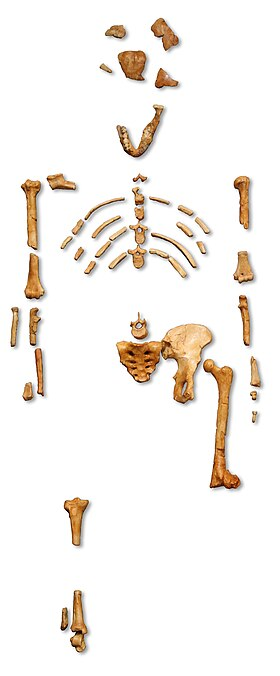
\includegraphics[width=1.8cm]{Lucy.jpg}}
    \dleft{13cm}{\item Découverte en 1991 en Italie, la momie d'Ötzi contenait 53,3 \% (à 1\% près) de C$_{14}$ par rapport à un homme vivant. Donner un encadrement de l'âge d'Ötzi.}
    {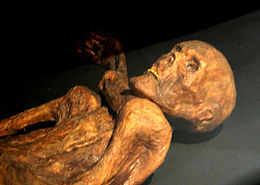
\includegraphics[width=2.8cm]{Otzi-Quinson.jpg}}
\end{enumerate}

\exo{}
\dleft{12cm}{
    Dans une réserve marine, on a recencé 3000 cétacés au 1$^{\text{er}}$ janvier 2020. Les responsables sont inquiets car le classement de la zone en « réserve marine » ne sera pas reconduit si le nombre de cétacés de cette réserve devient inférieur à 2000.\\
    Une étude permet d'élaborer un nodèle selon lequel :
}
{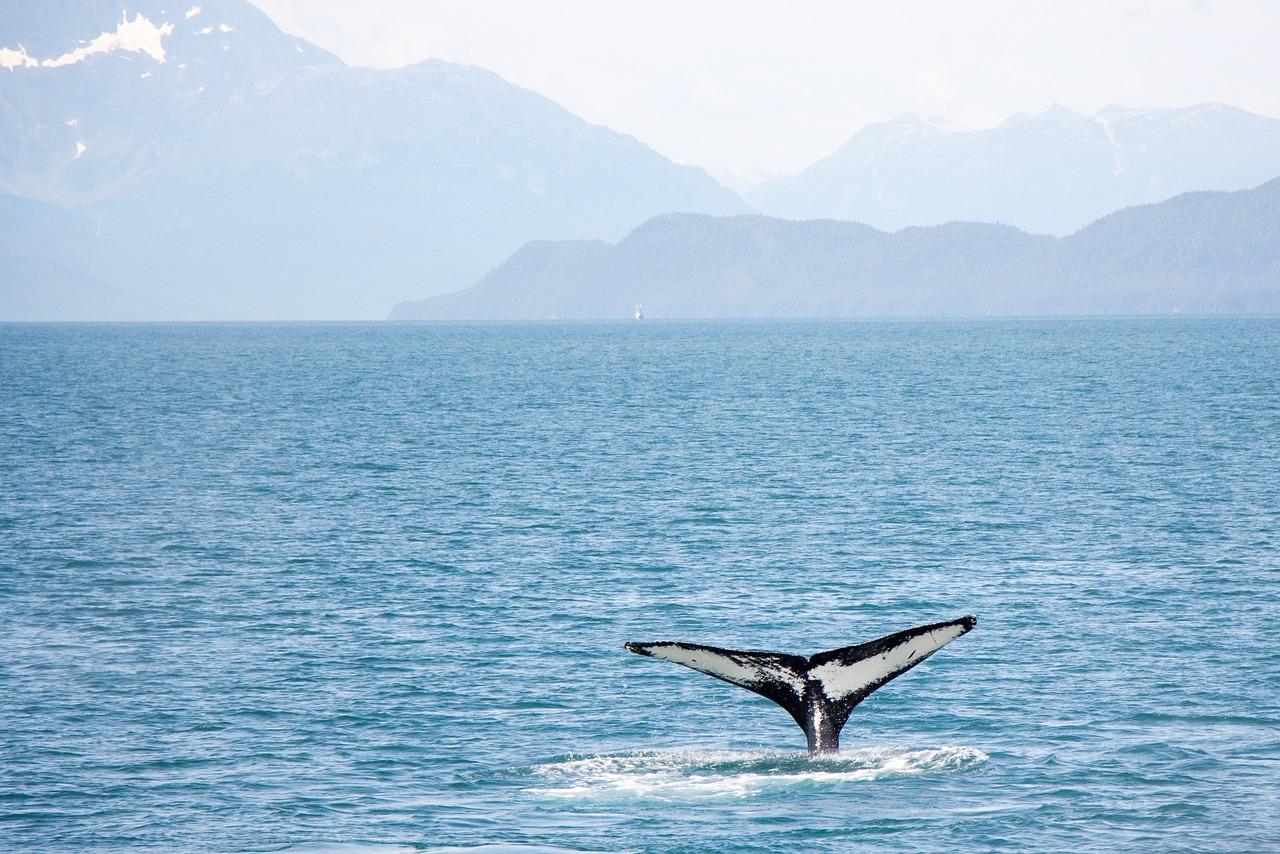
\includegraphics[width=4.2cm]{whale-4424846_1280.jpg}}
\begin{enumerate}[label=\textbullet]
    \item entre le 1$^{\text{er}}$ juin et le 31 octobre, 80 cétacés arrivent dans la réserve marine ;
    \item entre le 1$^{\text{er}}$ novembre et le 31 mai, la réserve subit une baisse de 5 \% de son effectif par rapport à celui du 31 octobre.
\end{enumerate}
On modélise le nombre de cétacés dans la réserve marine au 1$^{\text{er}}$ juin de l'année 2020 $+n$ par le terme $u_n$. Ainsi $u_0=3000$.
\begin{enumerate}
    \item Justifier que $u_1=2926$.
    \item Justifier que pour tout $n\in\N$, $u_{n+1}=0,95u_n+76$.
    \item Démontrer que pour tout $n\in\N$, $u_{n}=1480\times 0,95^n+1520$.
    \item Déterminer la limite de la suite $(u_n)$.
    \item La réserve marine fermera-elle ? Si oui, en quelle année ? \textit{Répondre à l'aide d'un calcul.}
\end{enumerate}
\newpage

\exo{}
Une agence bancaire propose un placement à tous ses clients. Ce placement a rapporté 30 \% d'intérêts sur les 5 dernières années.\\
On note $t$ \% le taux d'intérêt annuel moyen de ce placement sur ces 5 dernières années.
\begin{enumerate}
    \item Justifier que le taux d'intérêt annuel moyen $t$ est tel que $1,3=\left(1+\dfrac{t}{100}\right)^5$.
    \item Résoudre l'équation précédente en utilisant la fonction logarithme népérien. \textit{Donner la valeur exacte, puis l'arrondi au centième.}
    \item Interpréter le résultat obtenu dans le contexte de la situation.
\end{enumerate}


\subsection*{Étude de la fonction logarithme népérien}

\exo{}
Dans chaque cas, donner la fonction dérivée de la fonction $f$ définie sur $\oio{0}{+\infty}$.
\begin{multicols}{3}
    \begin{enumerate}
        \item $f(x)=5\ln(x)$
        \item $f(x)=3-2\ln(x)$
        \item $f(x)=x\ln\left(x\right)-1$
        \item $f(x)=\ln(2x)$
        \item $f(x)=\ln\left(x^2\right)$
        \item $f(x)=\ln\left(3x^2+1\right)$
    \end{enumerate}
\end{multicols}

\exo{}
Soit $f$ la fonction définie sur $\oio{0}{+\infty}$ par $f(x)=\ln x +x$.
\begin{enumerate}
    \item Déterminer les limites de $f$ aux bornes de son ensemble de définition.
    \item Calculer la dérivée de $f$ et dresser le tableau de variation de $f$ sur $\oio{0}{+\infty}$.
\end{enumerate}

\exo{}
Soit $f$ la fonction définie sur $\oio{0}{+\infty}$ par $f(x)=-\dfrac{1}{x}+\ln x$.
\begin{enumerate}
    \item Déterminer les limites de $f$ aux bornes de son ensemble de définition.
    \item Calculer la dérivée de $f$, en déduire son sens de variation sur $\oio{0}{+\infty}$ et son signe.
\end{enumerate}

\newpage

\exo{}
Soit $f$ la fonction définie sur $\oio{0}{14}$ par $f(x)=2-\ln \left(\dfrac{x}{2}\right)$.\\[.5em]
La courbe représentative $\mathcal{C}_f$ de la fonction $f$ est donnée dans le repère orthonormé ci-dessous.
\begin{center}
    \def\xmin{-1} \def\ymin{-1}\def\xmax{15}\def\ymax{5}
        \begin{tikzpicture}[scale=.7]
            \clip (\xmin,\ymin) rectangle (\xmax,\ymax);
            \draw[fill = white] (\xmin,\ymin) rectangle (\xmax,\ymax);
            \coordinate (M) at (1.7,2.16);
            \draw[UGLiOrange] (M) node[above]{$M$};
            \fill[UGLiOrange] (0,0) -- (1.7,0) -- (M) -- (0,2.16) ;
            \draw[UGLiOrange] (1.7,0) node[below]{$P$};
            \draw[UGLiOrange] (0,2.16) node[left]{$Q$};
            \repereal{\xmin}{\ymin}{\xmax}{\ymax}
            \draw[color=UGLiRed,thick,samples=1000,domain=0.01:14,smooth,variable=\x] plot ({\x},{2-ln(\x/2)});
            
            
        \end{tikzpicture}
\end{center}
À tout point $M$ appartenant à $\mathcal{C}_f$, on associe le point $P$ projeté orthogonal de $M$ sur l'axe des abscisses et le point $Q$ projeté orthogonal de $M$ sur l'axe des ordonnées.
\begin{enumerate}
    \item Montrer que la fonction $g:x\mapsto 2x-x\ln \left(\dfrac{x}{2}\right)$ modélise l'aire du rectangle $OPMQ$.
    \item Dresser le tableau de variation de $g$ sur $\oio{0}{14}$.
    \item En déduire les coordonnées du point $M$ pour lesquelles l'aire du rectangle $OPMQ$ est maximale.
    On admettra que $\lim\limits_{x\to 0^+} g(x)=0$.
\end{enumerate}

\exo{}%Hyperbole p 113
\dleft{12cm}{
\begin{encadrecolore}{Un peu d'histoire}{UGLiDarkBlue}
    Durant la Renaissance, le commerce se développant, les marchands ont été amenés à constituer des tables d'intérêts pour faciliter les calculs financiers. \textbf{Luca Pacioli} (1445-1517), religieux franciscain, mathématicien et fondateur de la comptabilité, présente la règle des 72 en 1494 dans son ouvrage \textit{Summa de arithmetica, geometria, proportioni et proportionalità}.\\
    Cette règle est une méthode pour estimer le temps de doublement d'un capital. Luca Pacioli estime que si un capital est placé à un taux d'intérêt annuel de $t$ \% alors il faut environ $\dfrac{72}{t}$ années pour le doubler.
\end{encadrecolore}}
{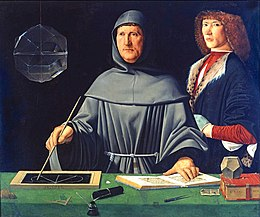
\includegraphics[width=4.2cm]{Pacioli.jpg}\\
\tiny{Portrait du mathématicien Luca Pacioli expliquant le théorème d'Euclide (oeuvre attribuée à Jacopo de Barbari, 1495).}}

\subsubsection*{Partie A : la règle des 72}
$t$ désigne un nombre réel strictement positif et $n$ est un nombre entier naturel non nul.
\begin{enumerate}
    \item Utiliser la règle de Pacioli pour estimer le nombre $n$ d'années nécessaires pour doubler un capital lorsqu'il est placé à un taux d'intérêts composés de :
    \begin{multicols}{3}
        \begin{enumerate}[label=\textbullet]
            \item $t=1$ \%
            \item $t=5$ \%
            \item $t=10$ \%
        \end{enumerate}
    \end{multicols}
    \item Au bout de $n$ années de placement au taux d'intérêt de $t$ \%, le capital est multiplié par $\left(1+\dfrac{t}{100}\right)^n$.
    \begin{enumalph}
        \item Dans chaque cas, déterminer, en utilisant la fonction $\ln$, le plus petit nombre entier naturel $n$ tel que $\left(1+\dfrac{t}{100}\right)^n\geqslant 2$.
        \begin{multicols}{3}
            \begin{enumerate}[label=\textbullet]
                \item $t=1$ \%
                \item $t=5$ \%
                \item $t=10$ \%
            \end{enumerate}
        \end{multicols}
        \item Comparer les résultats obtenus dans les questions 1 et 2.
    \end{enumalph}
\end{enumerate}

\subsubsection*{Partie B : une autre estimation}
\begin{enumerate}
    \item $f$ et $g$ sont les fonctions définies sur l'intervalle $\fio{0}{+\infty}$ par $\quad f(x)=\ln(1+x)-x+\dfrac{x^2}{2}\quad$ et $\quad g(x)=\ln (1+x)-x$.
    \begin{enumalph}
        \item Étudier les variations de $f$ et $g$ sur $\fio{0}{+\infty}$.
        \item En déduire que pour tout réel $x$ de l'intervalle $\fio{0}{+\infty}$, $\quad x-\dfrac{x^2}{2}\leqslant \ln(1+x)\leqslant x$.
    \end{enumalph}
    \item Pour des petites valeurs de $x$, $\dfrac{x^2}{2}$ étant très petit, on choisit d'utiliser l'approximation $\ln(1+x)\approx x$.
    \begin{enumalph}
        \item Justifier que le nombre de périodes nécessaires au doublement d'un capital placé à un taux d'intérêt annuel de $t$ \% est proche de $\dfrac{70}{t}$ (pour des petites valeurs de $t$).
        \item Que devient cette règle si l'on veut tripler le capital ?
    \end{enumalph}
\end{enumerate}
\end{document}